\chapter{Metodologia}\label{ch:metodologia}

A metodologia desse projeto será dividida em quatro fases: sistema mecânico, sistema eletrônico, 
desenvolvimento do sistema de software e integração dos sistemas.

\section{Sistema mecânico}\label{sec:metmecanico}

Nesta seção será desenvolvido o projeto do sistema mecânico que se divide em estrutura e componentes. 
Para compreensão facilitada do projeto, os cálculos de resistência e equilíbrio foram desconsiderados, 
já que o equipamento é de pequena escala.

\subsection{Estrutura}\label{subsec:metestrutura}

A estrutura ou mesa cartesiana, como é chamada neste trabalho, compõem o sistema mecânico junto com seus 
componentes, é a parte responsável por manter a união das peças que ela a compõem e também servir de base 
para o posicionamento dentro da área de testes do túnel de vento. Como o túnel de vento do Laboratório de 
Sistemas Térmicos da Universidade Federal do Rio Grande é utilizado para atividades de pesquisa em energia 
renovável e fenômenos de transporte, optou-se por projetar uma estrutura móvel, que pode ser colocada e 
retirada de dentro do túnel, quando há a necessidade da caracterização do canal aberto. Para que essa 
operação se torne prática a mesa deve ser leve e resistente.

Por ser um metal leve, durável e resistente, o alumínio se torna uma boa opção para a confecção desta 
estrutura. Com uma alta relação resistência/peso, confere um excepcional desempenho, além de dar um ótimo 
acabamento à peça. A estrutura de metal será dividida em duas partes, a base e o pórtico. A base será 
o componente que terá a função de dar estabilidade a mesa e evitar que esta venha a tombar, terá um 
formato retangular de 500~x~400~mm e será feito com um perfil V-Slot de 20~x~40~mm em alumínio, conforme 
apresentado na Figura \ref{fig:p20x40p}. 
Para fazer a união dos perfis, que serão cortados em tamanho adequado com cantos esquadrejados em 
ângulo de 45°, para dar um melhor acabamento à peça, será utilizada uma placa de conexão 
interna de 90°, conforme a Figura \ref{fig:pconexao90p}, que unirá os cantos dos perfis por 
meio de parafusos Allen sem cabeça com rosca M5.
    
\begin{figure}[H]
\centering
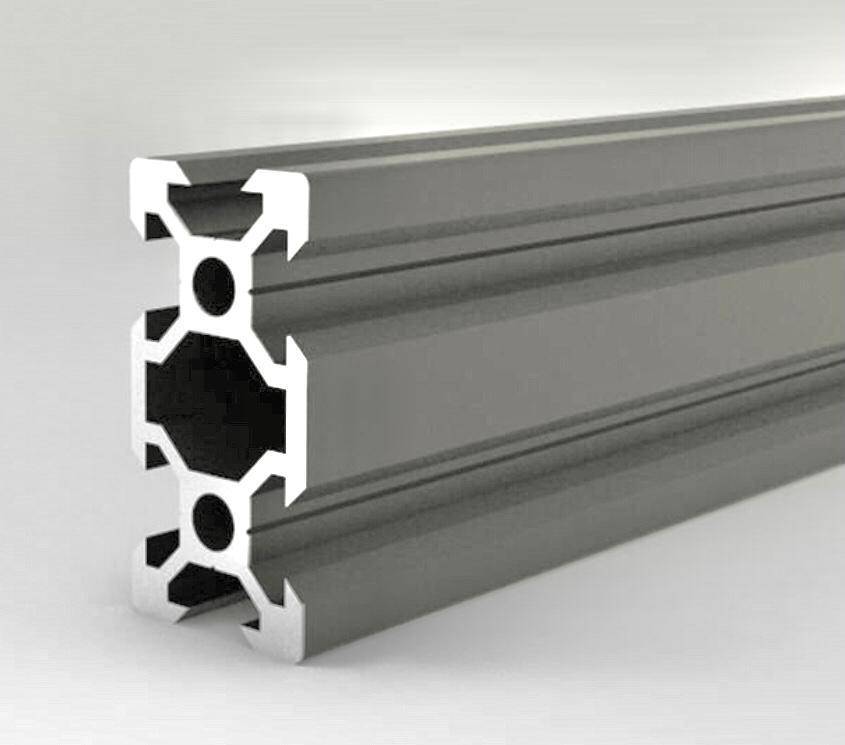
\includegraphics[scale = 0.3]{figuras/p20x40p2}
\caption{Perfil V-slot  20~x~40~mm em alumínio.}
\caption*{Fonte: www.forsetisolucoes.com.br}
\label{fig:p20x40p}
\end{figure}
    
\begin{figure}[H]
\centering
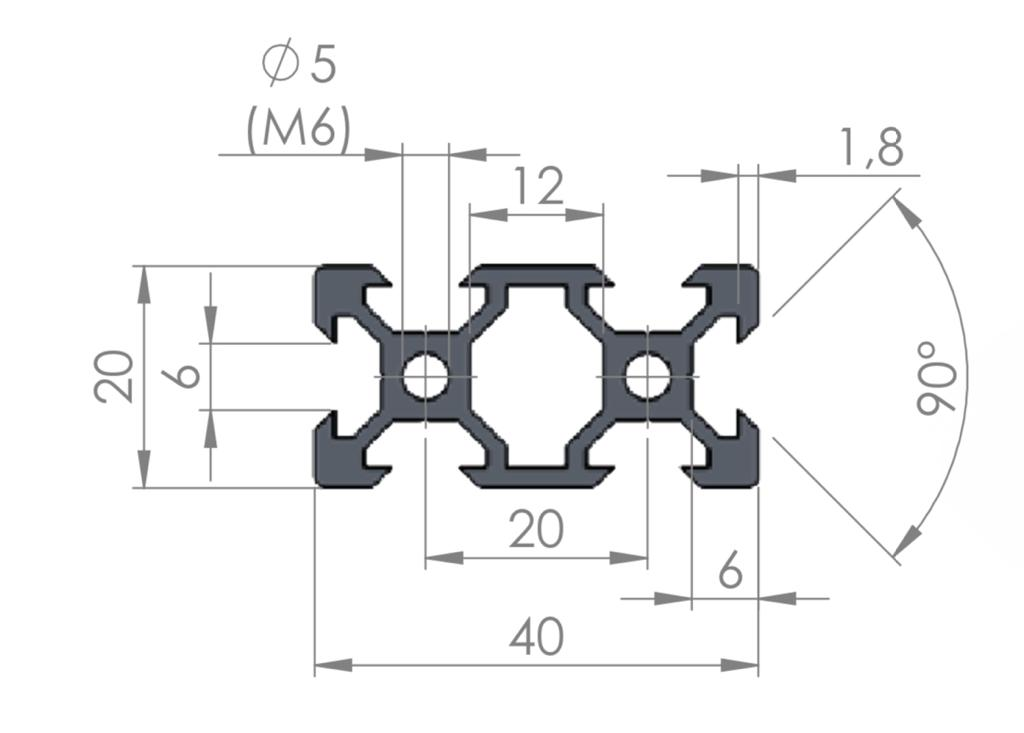
\includegraphics[scale = 0.4]{figuras/p20x40d}
\caption{Dimensões do perfil 20~x~40~mm.}
\caption*{Fonte: www.forsetisolucoes.com.br}
\label{fig:p20x40d}
\end{figure}
    
\begin{figure}[H]
\centering
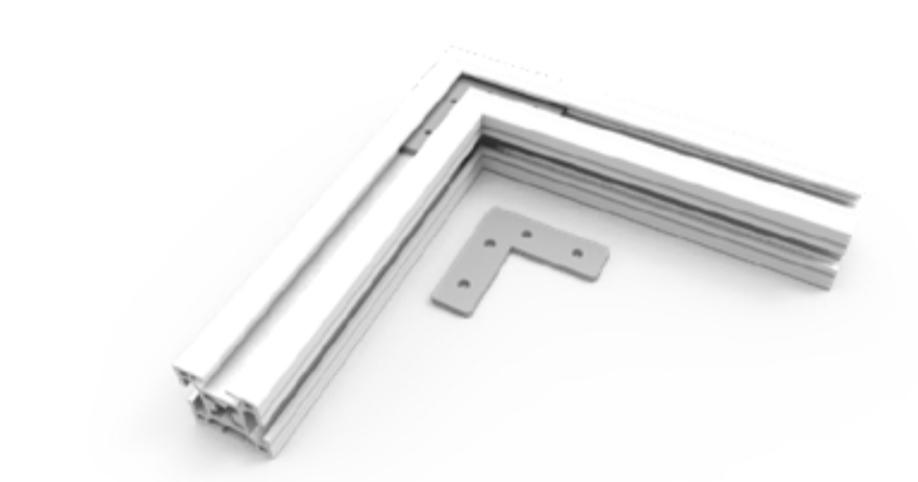
\includegraphics[scale = 0.4]{figuras/pconexao90p}
\caption{Placa de conexão interna de 90°.}
\caption*{Fonte: www.forsetisolucoes.com.br}
\label{fig:pconexao90p}
\end{figure}
    
\begin{figure}[H]
\centering
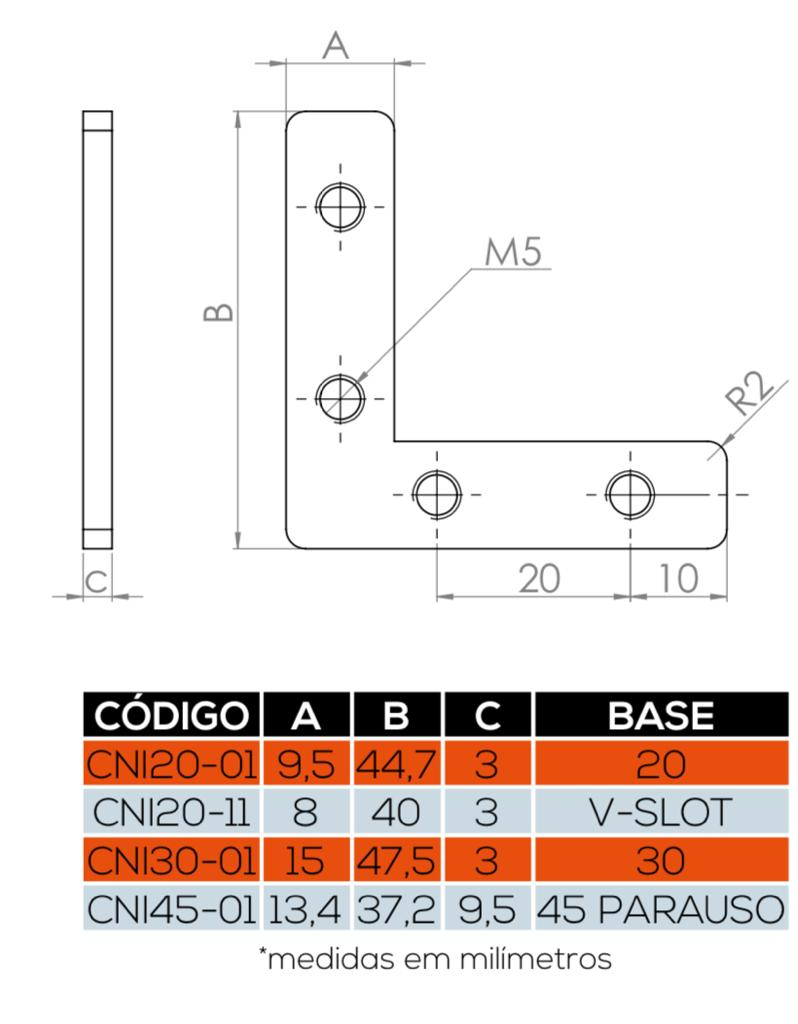
\includegraphics[scale = 0.4]{figuras/pconexao90d}
\caption{Dimensões da placa de conexão interna de 90°.}
\caption*{Fonte: www.forsetisolucoes.com.br}
\label{fig:pconexao90d}
\end{figure}

\begin{figure}[H]
\centering
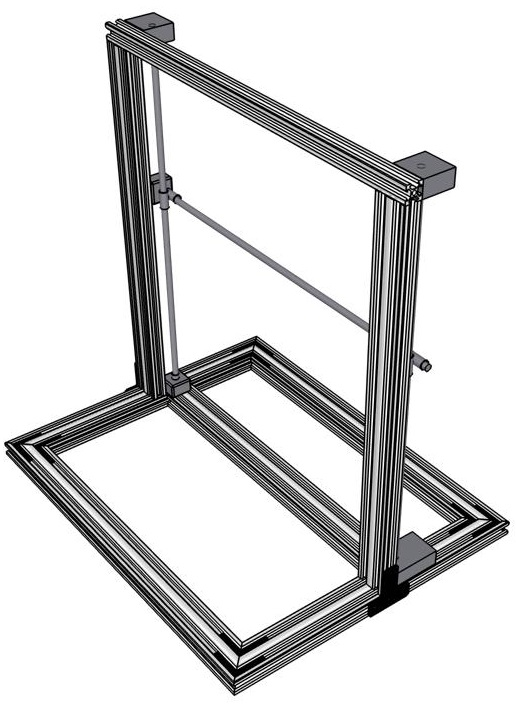
\includegraphics[scale = 1]{figuras/estruturamesa}
\caption{Esboço da mesa cartesiana.}
\caption*{Fonte: Próprio autor}
\label{fig:estruturamesa}
\end{figure}

\begin{figure}[H]
\centering
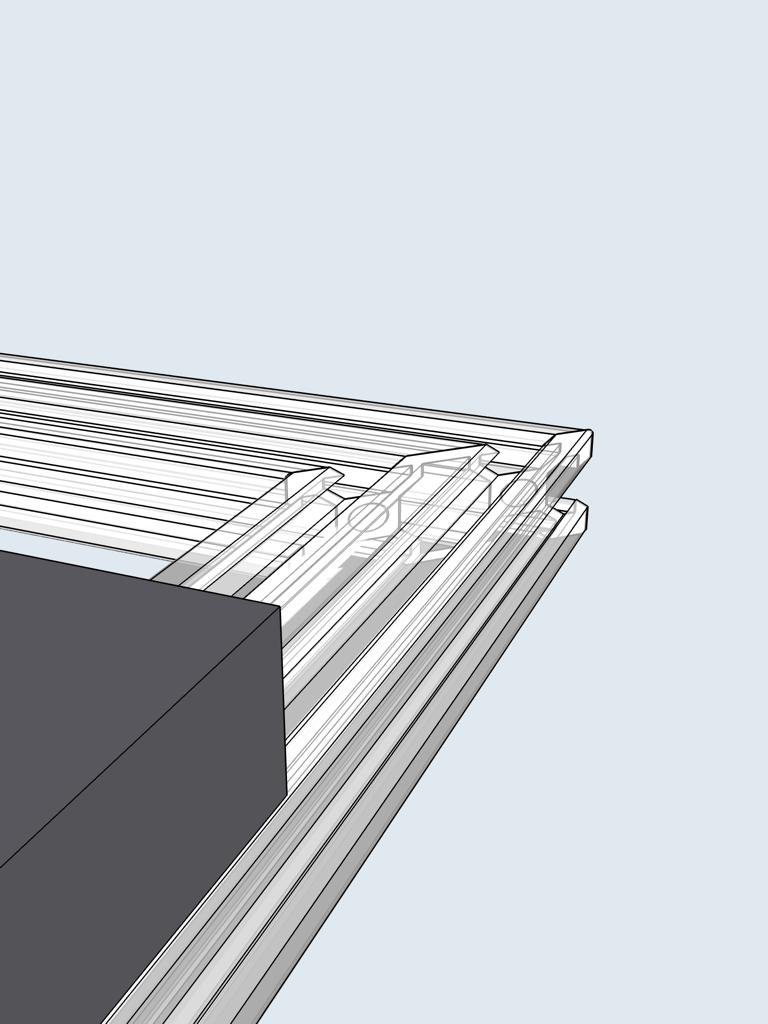
\includegraphics[scale = 0.5]{figuras/detalhe45}
\caption{Detalhe do encaixe a 45° da base da estrutura.}
\caption*{Fonte: Próprio autor}
\label{fig:detalhe45}
\end{figure}
    
O pórtico será feito com o perfil V-Slot de 20~x~20~mm em alumínio conforme apresenta 
a Figura \ref{fig:p20x20p}, e terá as dimensões de 500~x~480~mm. Sua função é sustentar 
e estabilizar o sistema de transmissão. Para fixação do pórtico à base será utilizada 
uma placa T simples de aço, fixada com parafusos Allen cabeça abaulada com rosca M6~x~10~mm 
e porca T reforçada com rosca M6. Na montagem da parte superior do pórtico a união 
se dará por meio de parafusos com rosca M6~x~16~mm diretamente nos perfis, para tanto, 
terá que ser feita uma rosca M6 nos furos dos perfis verticais V-Slot 20~x~40~mm para 
fixação dos parafusos e furos de 5~mm no perfil horizontal do pórtico para que se 
possa acessar e realizar o aperto desses parafusos com chave Allen de 4~mm realizando 
assim uma união resistente entre os perfis.

%DA PRA COLOCAR FOTO

\begin{figure}[H]
\centering
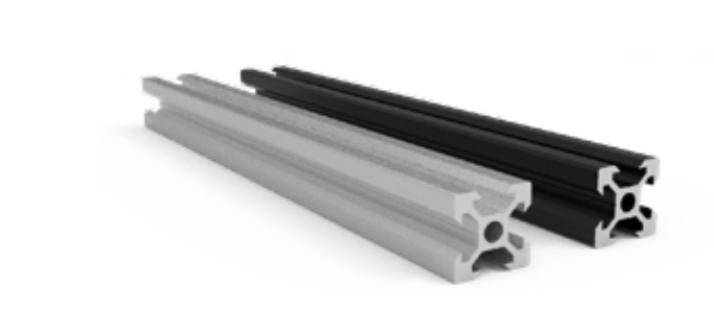
\includegraphics[scale = 0.4]{figuras/p20x20p}
\caption{Perfil V-Slot 20~x~20~mm em alumínio.}
\caption*{Fonte: www.forsetisolucoes.com.br}
\label{fig:p20x20p}
\end{figure}
    
\begin{figure}[H]
\centering
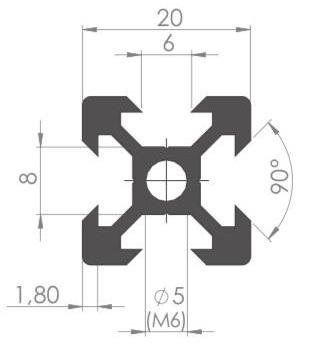
\includegraphics[scale = 1]{figuras/p20x20d}
\caption{Dimensões do perfil 20~x~20~mm.}
\caption*{Fonte: www.forsetisolucoes.com.br}
\label{fig:p20x20d}
\end{figure}
    
\begin{figure}[H]
\centering
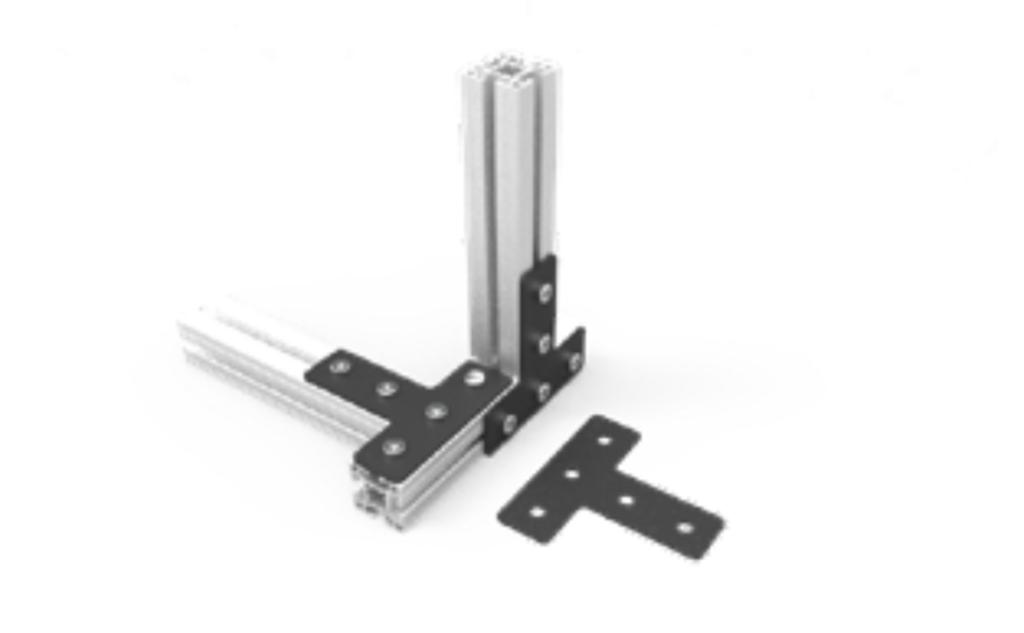
\includegraphics[scale = 0.4]{figuras/placatp}
\caption{Placa T simples de aço.}
\caption*{Fonte: www.forsetisolucoes.com.br}
\label{fig:placatp}
\end{figure}
    
\begin{figure}[H]
\centering
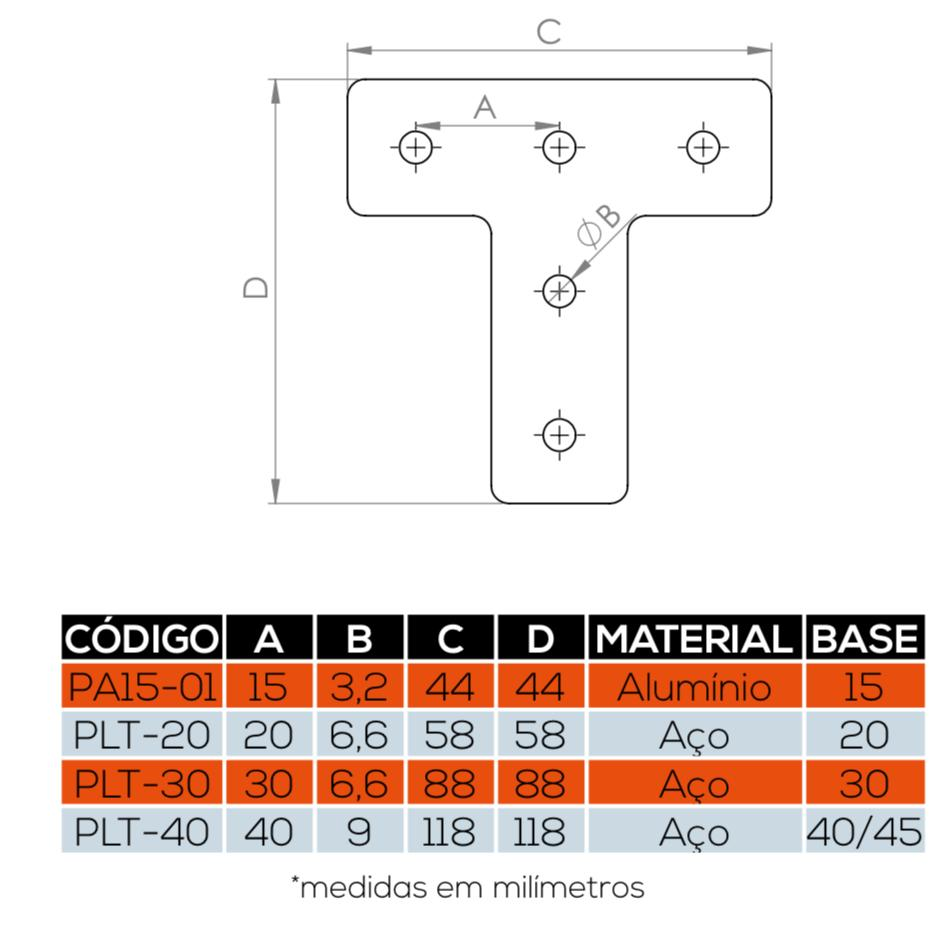
\includegraphics[scale = 0.4]{figuras/placatd}
\caption{Dimensões da placa T simples.}
\caption*{Fonte: www.forsetisolucoes.com.br}
\label{fig:placatd}
\end{figure}

\subsection{Sistema de transmissão}\label{subsec:mettransmissao}

%PRECISA COLOCAR REFERENCIA \cite{budynas2016elementos}
Segundo \citeauthor{budynas2016elementos} (\citeyear{budynas2016elementos}), o parafuso de potência 
é um dispositivo usado para transformar o movimento angular em movimento linear e, usualmente, 
para transmitir potência. Para fazer o movimento dos carros do eixo X e do eixo Y, 
componentes que farão o efetivo deslocamento do equipamento de medição dentro da área de 
teste do túnel de vento, o fuso foi escolhido como elemento de transmissão, que vai transformar 
o movimento giratório do motor de passo em deslocamento linear na estrutura da mesa cartesiana. 
Acoplados aos motores de passo, por meio de acopladores de eixo e na outra extremidade por mancal para fuso 
de 8~mm, os fusos farão o transporte dos carros horizontal e vertical. 

Para que se tenha um deslocamento mais rápido das castanhas, elemento que estará em contato 
direto com o fuso e o carro, foi selecionado o fuso TR8~x~8~mm com 4 entradas que é um fuso trapezoidal 
de 8~mm de diâmetro e 2~mm de passo com um avanço de 8~mm. A elevação do sistema de medição será 
executada por dois fusos paralelos. Para o deslocamento horizontal será utilizado um fuso TR8~x~8~mm 
acoplado a um motor de passo junto com uma haste guia para dar sustentação e evitar que o sistema 
de medição gire em torno do eixo.

\subsection{Acionador}\label{subsec:metacionador}

Os motores elétricos são máquinas capazes de transformar energia elétrica em energia mecânica, 
essa energia se dá em forma de movimento angular. São equipamentos versáteis, muito eficientes 
e amplamente utilizados. Para fazer a movimentação dos carros, nos eixos X e Y, optou-se por 
motores de passo, por que é um motor que possibilita o controle da velocidade e o posicionamento 
preciso, pois rotaciona em ângulos bem definidos, chamados de passos. O ponto negativo desses 
motores é que o controle é mais complexo, necessitando de um comando eletrônico digital para 
fazê-lo funcionar, por outro lado apresenta uma grande precisão no seu movimento. Os motores 
serão acoplados aos perfis da estrutura de modo a possibilitar o movimento dos fusos e consequentemente 
o equipamento de medição, que estará preso a ele por meio de uma guia com roldana. 

\subsection{Cálculo dos esforços sobre a haste e o fuso}\label{subsec:metcalculos}

As forças envolvidas para erguer a carga e fazer o deslocamento do tubo de Pitot na direção horizontal 
são baixas, não havendo necessidade de se fazer um cálculo estrutural, porém por se tratar de 
um projeto mecânico, é inevitável que se tenha a garantia de que a estrutura resista aos 
esforços mecânicos. Para tanto serão feitos cálculos para obter valores máximos de esforços 
e compará-los com os valores admissíveis.

Os cálculos a seguir serão fundamentados nos livros \citeauthor{juvinall2020fundamentals} (\citeyear{juvinall2020fundamentals}) e \citeauthor{budynas2016elementos} (\citeyear{budynas2016elementos}).

\subsubsection{Cálculo da máxima deflexão}

Para os cálculos, foi considerado o Aço inoxidável 303, por segurança, pois o fabricante da haste e do fuso 
não especifíca o material.

Dados: 
$E_{Aco}~=~190~GPa$ de acordo com o \citeauthor{juvinall2020fundamentals} (\citeyear{juvinall2020fundamentals}),\\
$d_{haste}~=~16~mm$, $L~=~400~mm$.

Onde:
\begin{itemize}
    \item $E_{Aco}$ é o Módulo de elasticidade do Aço;
    \item $d_{haste}$ é o diâmetro da haste;
    \item $L$ é o comprimento da haste.
\end{itemize}

Considerações:
\begin{itemize}
    \item Considerando apoios simples com carga central;
    \item Deflexão máxima = 0,05~mm.
\end{itemize}

A equação \ref{eq:momentodeinercia} calcula o momento de inércia segundo o \citeauthor{juvinall2020fundamentals} (\citeyear{juvinall2020fundamentals}).
\begin{equation}\label{eq:momentodeinercia}
    I = \frac{\pi \cdot d^{4}}{64}
\end{equation}

Utilizando a equação \ref{eq:momentodeinercia} se obtém o momento de inércia da haste.

$$I_{h} = \frac{\pi \cdot (8~mm)^{4}}{64} = 3216,990877~mm^{4}$$   

A Figura \ref{fig:diagramacorpolivre} mostra o diagrama de corpo livre da haste.

\begin{figure}[H]
\centering
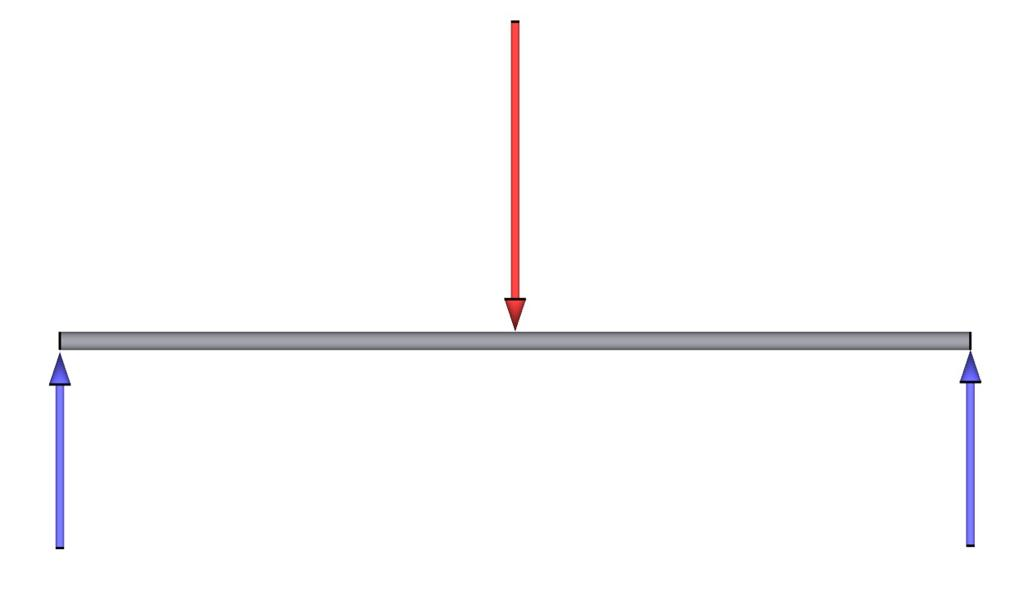
\includegraphics[scale = 0.4]{figuras/diagramcorpolivre}
\caption{Diagrama de corpo livre da haste.}
\caption*{Fonte: Próprio autor}
\label{fig:diagramacorpolivre}
\end{figure}

A equação \ref{eq:deflexao} calcula a deflexão segundo o \citeauthor{budynas2016elementos} (\citeyear{budynas2016elementos}).
\begin{equation}\label{eq:deflexao}
    Y_{max} = \frac{F \cdot L^{3}}{48 \cdot E \cdot I}
\end{equation}

Utilizando a equação \ref{eq:deflexao} se obtém a força máxima para a deflexão de $0,05~mm$, 
para isso foi utilizado o momento de inércia da haste.

$$F = \frac{0,05~mm \cdot 48 \cdot 190 \cdot 10^{3}~\frac{N}{mm^{2}} \cdot 3216,990877~mm^{4}}{(400~mm)^{3}} = 22,92106~N$$

\subsubsection{Cálculo da força máxima suportada pelo fuso}

A Figura \ref{fig:esqforcafuso} mostra esquematicamente a força agindo sobre a castanha e consequentemente 
sobre os dentes do fuso.

\begin{figure}[H]
\centering
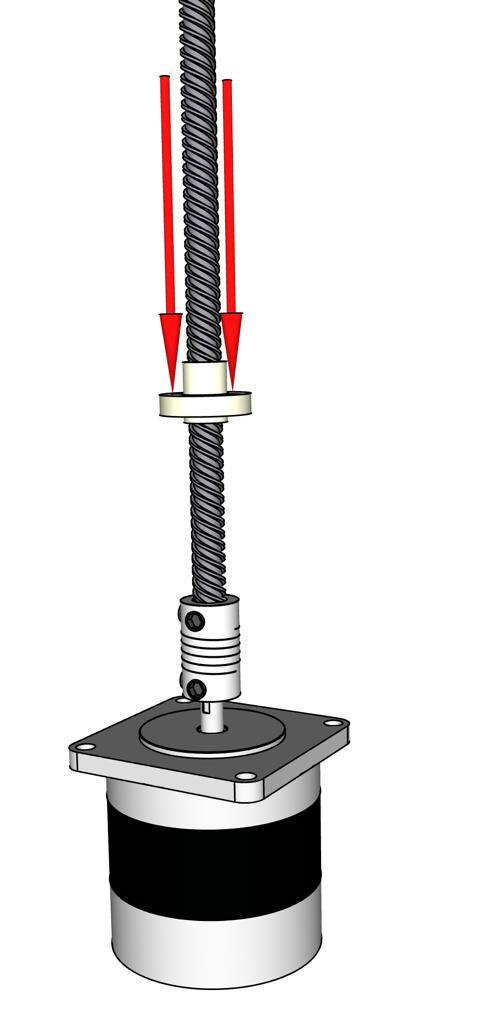
\includegraphics[scale = 0.25]{figuras/esqforcafuso}
\caption{Força agindo sobre o fuso.}
\caption*{Fonte: Próprio autor}
\label{fig:esqforcafuso}
\end{figure}
    
Dados:
$d_{m} = 8~mm$, $P = 2~mm$

Onde:
\begin{itemize}
    \item $d_{m}$ é o diâmetro médio;
    \item $P$ é o passo;
    \item $L_{a}$ é o avanço que é igual ao número de entradas vezes o passo;
    \item $T$ é o torque do motor (Datasheet).
\end{itemize}

A equação \ref{eq:dmedio} calcula o diâmetro médio segundo o \citeauthor{budynas2016elementos} (\citeyear{budynas2016elementos}).
\begin{equation}\label{eq:dmedio}
    d_{m} = d - \frac{P}{2}
\end{equation}

Utilizando a equação \ref{eq:dmedio} se obtém o diâmetro médio considerando $d_{m} = 8~mm$:

$$d_{m} = 8~mm - \frac{2}{2}~mm = 8~mm - 1~mm = 7~mm$$

A equação \ref{eq:avanco} calcula o avanço.
\begin{equation}\label{eq:avanco}
    L_{a} = n_{e} \cdot P = 8~mm
\end{equation}

Onde:
\begin{itemize}
    \item $L_{a}$ é o avanço;
    \item $n_{e}$ é o número de entradas;
    \item $P$ é o passo.
\end{itemize}

Utilizando a equação \ref{eq:avanco} se obtém o avanço considerando o número de entrada igual a 4 e o passo igual $2~mm$:
$$L_{a} = 4 \cdot 2 = 8~mm$$ 

Considerando o torque do motor conforme o \textit{datasheet}.
$$T = 5~kgf \cdot cm = 490,33~N \cdot mm$$

\begin{equation}\label{eq:torque}
T = \frac{F \cdot d_{m}}{2} \cdot (\frac{L_{a} + \pi \cdot f \cdot d_{m}}{\pi \cdot d_{m} - f \cdot L_{a}}) + \frac{F \cdot f_{c} \cdot d_{c}}{2}
\end{equation}

Admitindo um coeficiente de fricção e coeficiente de fricção no colar igual a 0,08.
$$f = f_{c} = 0,08$$

Onde:
\begin{itemize}
    \item $f$ é o coeficiente de fricção;
    \item $f_{c}$ é o coeficiente de fricção no colar;
    \item $d_{c}$ é o diametro do colar.
\end{itemize}

Considerando o $d_{c}$ = 0

$$490,33~N \cdot mm = \frac{F \cdot 7~mm}{2} \cdot (\frac{8~mm + \pi \cdot 0,08 \cdot 7~mm}{\pi \cdot 7~mm - 0,08 \cdot 8~mm})$$

$F = 306,55~N$

\subsubsection{Tensões de corpo}

A Figura \ref{fig:forcadente} mostra a força causando a flexão e o cisalhamento transversal na raiz da rosca.

\begin{figure}[H]
\centering
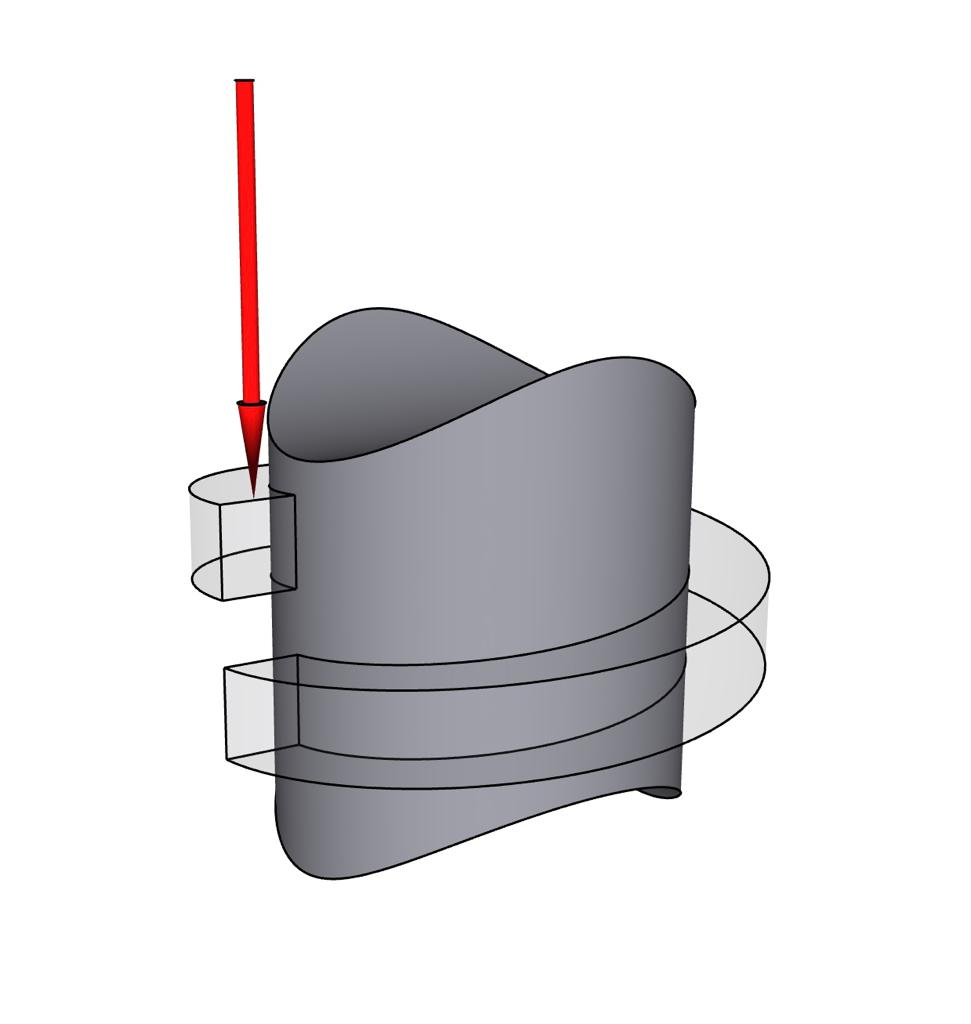
\includegraphics[scale = 0.2]{figuras/forcadente}
\caption{Força agindo sobre o dente.}
\caption*{Fonte: Próprio autor}
\label{fig:forcadente}
\end{figure}

Torcionais:

Tensão de cisalhamento devido ao momento de torção no lado externo do corpo do fuso.

\begin{equation}\label{eq:tensaocilhamento}
\tau = \frac{16 \cdot T}{\pi \cdot d_{r}^{3}}
\end{equation}

Onde:
$d_{r}$ é o diâmetro menor.
$$d_{r} = d - P = 8~mm - 2~mm = 6~mm$$

$$\tau = \frac{16 \cdot 490,33~N \cdot mm}{\pi \cdot (6~mm)^{3}} = 11,56~MPa$$

Tensões compressiva ou normal axial:

$$\sigma = - \frac{4 \cdot F}{ \pi (d_{r})^{2}}$$

$$\sigma = - \frac{4 \cdot 306,55~N}{ \pi (6~mm)^{2}} = -10,84~\frac{N}{mm^{2}}$$

\subsubsection{Tensão de sustentação}

Considerações:
\begin{itemize}
    \item A tensão de sustentação com uma rosca carregando 0,38~F;
    \item Número de roscas engajadas é igual a 1;
\end{itemize}

Onde:
\begin{itemize}
    \item $n_{t}$ é o número de roscas engajadas;
\end{itemize}

$$\sigma = \frac{2 \cdot (0,38 \cdot F)}{\pi \cdot d_{m} \cdot n_{t} \cdot P}$$

$$\sigma = \frac{2 \cdot (0,38 \cdot 306,55~N)}{\pi \cdot 7~mm \cdot 1 \cdot 2~mm} = 5,29~MPa$$

\subsubsection{Tensão de flexão da raiz da rosca}

\begin{equation}\label{eq:tensaoflexaoraizrosca}
\sigma_{raiz} = \frac{6 \cdot (0,38 \cdot F)}{\pi \cdot d_{r} \cdot n_{t} \cdot P}
\end{equation}

Utilizando a equação \ref{eq:tensaoflexaoraizrosca} se obtém a tensão de flexão da raiz da rosca:

$$\sigma_{raiz} = \frac{6 \cdot (0,38 \cdot 306,55)~N}{\pi \cdot 6~mm \cdot 1 \cdot 2~mm} = 18,5~MPa$$

\subsubsection{Tensão de Von Mises e tensão de cisalhamento máximo}

\begin{equation}\label{eq:vonmises}
\sigma_{2}, \sigma_{3} = \frac{\sigma_{x} + \sigma_{y}}{2} \pm \sqrt{(\frac{\sigma_{x} - \sigma_{y}}{2})^2 + \tau_{xy}^{2}}
\end{equation}

Utilizando a equação \ref{eq:vonmises} se obtém a tensão de cisalhamento máximo:

$$\sigma_{2}, \sigma_{3} = \frac{-10,82}{2} \pm \sqrt{(\frac{-10,82}{2})^2 + 11,56^{2}}$$

$$\sigma_{2} = 7,42~MPa$$
$$\sigma_{3} = -18,26~MPa$$

Logo:

$$\sigma_{1} = 18,5~MPa$$
$$\sigma_{2} = 7,42~MPa$$
$$\sigma_{3} = -18,26~MPa$$

A tensão de Von Mises:
\begin{equation}
\sigma' = (\frac{(\sigma_{1} - \sigma_{2})^{2} + (\sigma_{2} - \sigma_{3})^{2} + (\sigma_{3} - \sigma_{1})^{2}}{2})^{\frac{1}{2}}
\end{equation}

$$\sigma' = (\frac{(18,5 - 7,42)^{2} + (7,42 - (-18,26)))^{2} + (-18,26 - 18,5)^{2}}{2})^{\frac{1}{2}} = 32,66~MPa$$

Tensão Máxima:
\begin{equation}\label{eq:tensaomaxima}
\sigma_{1-3} = \frac{\sigma_{1} - \sigma{3}}{2}
\end{equation}

$$\sigma_{1-3} = \frac{18,5 - (-18,26)}{2} = 18,33~MPa$$

\section{Sistema eletrônico}\label{sec:metsisele}

O sistema eletrônico de uma mesa cartesiana foi dividido em módulos para um melhor detalhamento: 
placa de prototipagem eletrônica Arduino, drivers de potência, atuadores elétricos, fonte de alimentação, 
optoacopladores, encoders e um computador. É importante lembrar que para menor custo do projeto optou-se 
pela criação de dispositivos.

\begin{figure}[H]
\centering
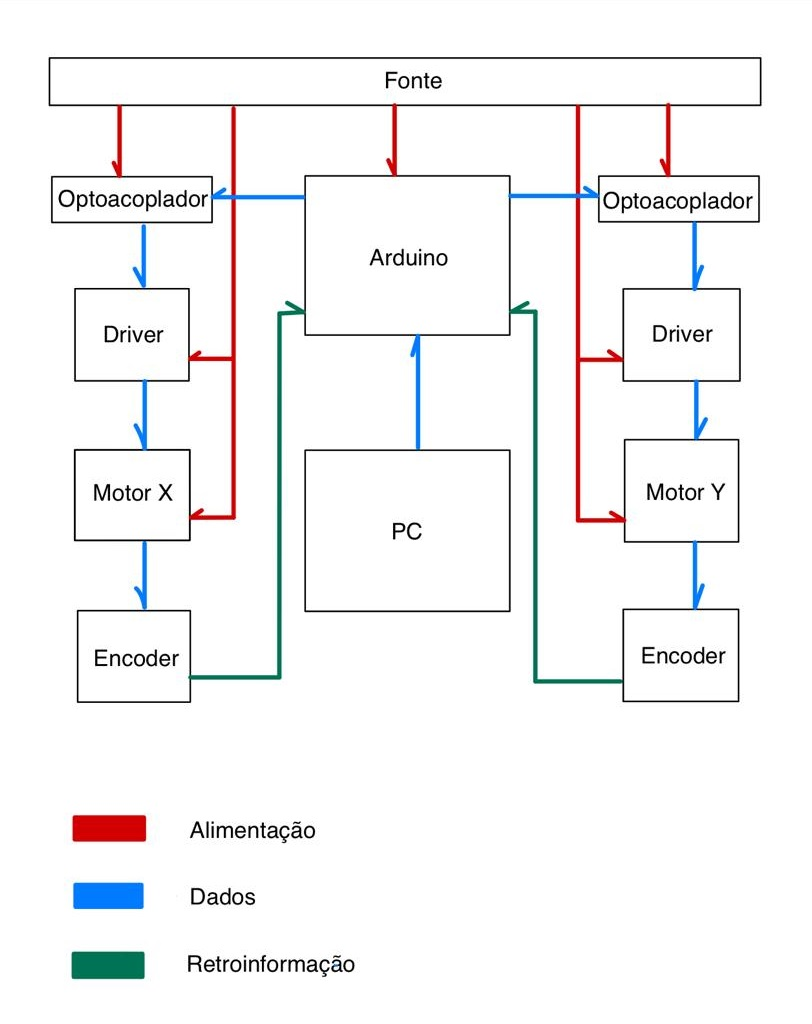
\includegraphics[scale = 0.6]{figuras/fluxogramaeletronico}
\caption{Fluxograma do sistema eletrônico.}
\caption*{Fonte: Próprio autor.}
\label{fig:fluxogramaeletronico}
\end{figure}
    
\subsection{Placa de prototipagem eletrônica Arduino}\label{subsec:metarduino}

A placa de prototipagem eletrônica Arduino é responsável pela recepção e tratamento dos dados provenientes 
da interface computacional. O controle dos motores está fundamentado na programação do microcontrolador 
de acordo com as necessidades definidas inicialmente para operação da mesa cartesiana.

Com o objetivo de elaborar uma interface de prototipagem de baixo custo para uso em projetos escolares, 
o arduino foi criado por um grupo de pesquisadores na Itália em 2005. Na sua concepção, para ter maior 
flexibilidade a diversos tipos de projetos, isto é, para que qualquer projetista pudesse personalizá-lo, 
foi adotado o conceito de hardware livre.

%ABREVIATURA DE RISC, PWM, RAM e EEPROM
Em sua composição, a placa Arduino UNO contém um microcontrolador ATMEL ATMEGA328, que é um dispositivo 
de 8 bits da família AVR com arquitetura \ac{RISC} avançada e com encapsulamento DIP28, além de quatorze portas 
digitais de entrada e saída, sendo que seis delas com capacidade de \ac{PWM}, seis 
entradas analógicas e 32 KB de memória flash, 2 KB de \ac{RAM} e 1 KB de \ac{EEPROM}. 

%ABREVIATURA DE USB
A alimentação é via porta \ac{USB} ou por conector tipo Jack de alimentação externa que trabalha entre os 
limites de 6~V e 20~V sendo recomendável o uso de 7~V a 12~V para não danificar. Para o fornecimento 
de tensão contínua para alimentação dos circuitos e Shields, a placa Arduino UNO tem um regulador 
de tensão de 3,3~V.

%ABREVIATURA DE USB
Além de alimentar, a porta \ac{USB} é a via de comunicação com o computador para o envio do código de máquina 
gerado pelo compilador. O código compilado é enviado pelo microcontrolador ATMEL ATMEGA16U2 que está 
conectado a dois LEDs chamados de TX e RX cuja função é a indicação do envio e recepção dos dados da 
placa para o computador.

%ABREVIATURA DE IDE
A placa Arduino é programada via \ac{IDE}, utilizando uma linguagem baseada em C/C++.

\begin{figure}[H]
\centering
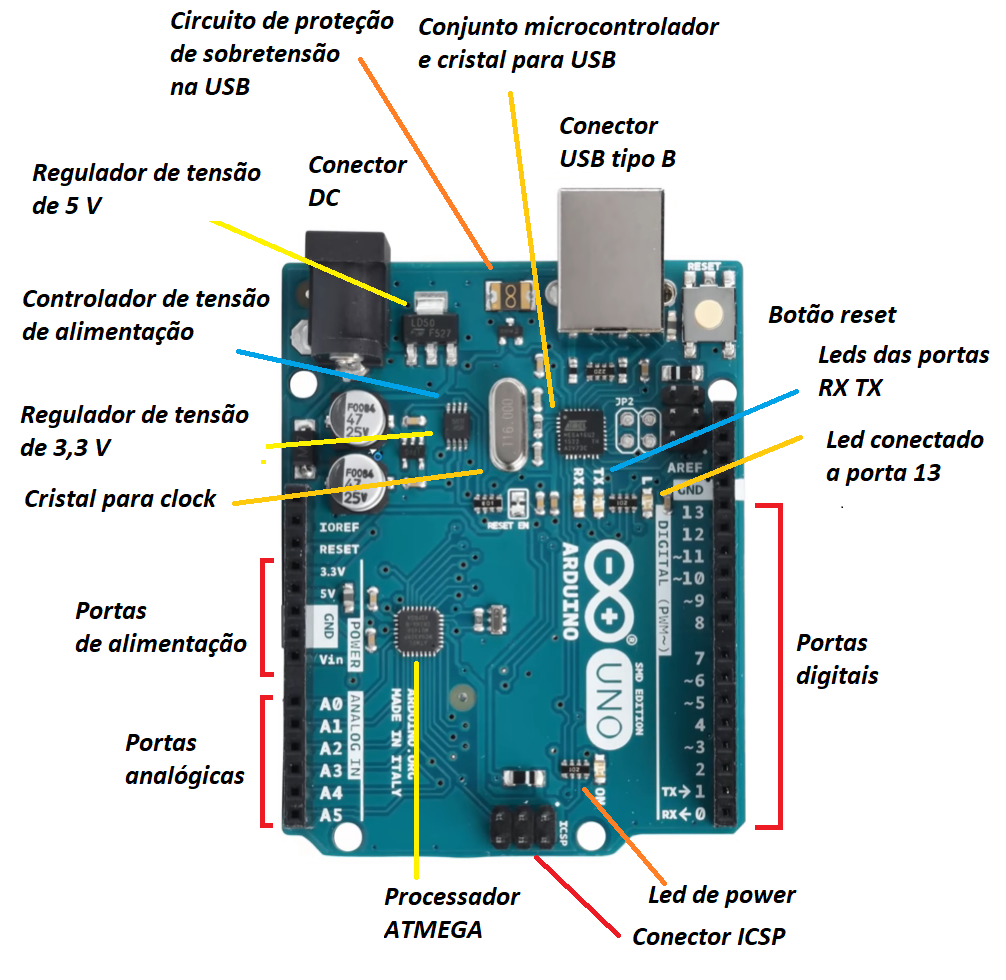
\includegraphics[scale = 0.6]{figuras/placaarduino}
\caption{Descrição dos componentes da placa Arduino.}
\caption*{Fonte: Próprio autor.}
\label{fig:placaarduino}
\end{figure}
    
\begin{itemize}
\item \textbf{Botão reset:} o botão reset serve para reiniciar a placa arduino.
\item \textbf{Conector \ac{USB} tipo B:} o conector \ac{USB} tipo B serve para conectar a placa Arduino ao computador.
\item \textbf{Conector DC:} o conector DC serve para alimentação externa do Arduino.
\item \textbf{Portas digitais:} são as portas que trabalham com os sinais digitais que são sinais com valores discretos, no arduino temos às constantes LOW que significa 0 V e também HIGH que significa 5 V, no código são 0 e 1 respectivamente. Dentro das portas digitais temos às portas \ac{PWM} que são portas que modulam o sinal pela largura do pulso, no arduino podemos variar de 0 a 255. Resumidamente, a placa Arduino possui quatorze portas digitais, sendo que seis delas são portas \ac{PWM} como dito anteriormente, os pinos delas são 3, 5, 6, 9, 10 e 11.
\item \textbf{Portas analógicas:} são as portas que trabalham com os sinais analógicos que são sinais com valores contínuos, no arduino podemos variar de 0 a 1023.
\item \textbf{Portas de alimentação:} são as portas de saída de tensão do arduino, temos três portas: porta 3,3~V cuja saída trabalha em 3,3~V, porta 5~V cuja saída trabalha em 5~V e a porta Vin cuja saída trabalha com a tensão de entrada do arduino.
\item \textbf{Led porta 13:} led conectado a porta 13 do arduino.
\item \textbf{Leds das portas RX TX:} leds conectados às portas RX TX, sendo que o led TX serve para indicar a transmissão de dados e o RX para indicar a recepção de dados.
\item \textbf{Processador ATMEGA328:} o processador é responsável pelo processamento da lógica de programação.
\item \textbf{Led de power:} led que acende quando o arduino está ligado.
\item \textbf{Conector \ac{ICSP}:} o conector \ac{ICSP}, que se refere a capacidade de programar Arduinos diretamente dos seus microcontroladores. 
\item \textbf{Conjunto microcontrolador e cristal para \ac{USB}:} esse conjunto possui um microcontrolador ATMEGA16U2 e um cristal externo de 16 MHz, e é responsável pelo gerenciamento da porta \ac{USB}.
\item \textbf{Circuito de proteção de sobretensão na \ac{USB}:} responsável por proteger a entrada \ac{USB} de sobretensão.
\item \textbf{Controlador de tensão de alimentação:} esse controlador é responsável por verificar se a tensão DC está presente, se não estiver, deixa que a tensão da \ac{USB} alimente o circuito. 
\item \textbf{Regulador de tensão de 5~V:} serve para regular a tensão em 5~V.
\item \textbf{Regulador de tensão de 3,3~V:} serve para regular a tensão em 3,3~V.
\item \textbf{Cristal para clock:} serve para gerar o clock.
\end{itemize}

\subsection{Drivers de potência}\label{subsec:metdriver}

Os drivers de potência são dispositivos que conservam sinais fundamentais de entrada em suas saídas, 
potencializando e fornecendo maior corrente elétrica para equipamentos atuadores. Os drivers de potência 
podem ser formados por elementos eletromecânicos (relés) e semicondutores (diodos, transistores, e 
circuitos integrados). 

No presente projeto, os drivers têm a função de, a partir dos sinais originados pelo Arduino, atender 
a demanda dos motores de passo utilizados.

A construção dos drivers que controlam os motores de passo da mesa cartesiana foi baseada em um 
circuito eletrônico para motores que trabalham com tensão de 12~V DC e até 10~A de corrente elétrica. 

\begin{figure}[H]
\centering
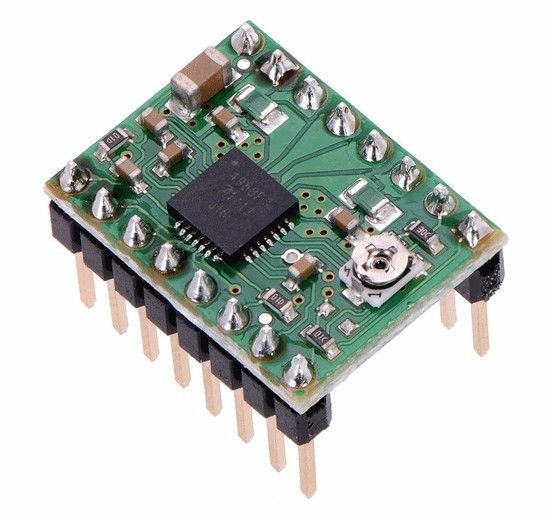
\includegraphics[scale = 0.4]{figuras/driver}
\caption{Driver A4988.}
\caption*{Fonte: https://www.eletrogate.com.}
\label{fig:driver}
\end{figure}

% Tabela 1
\begin{table}[H]
    \footnotesize
    \centering
    \caption{Parâmetros do driver de potência.}
    \begin{tabular}{ll}
        \hline
        \textbf{Parâmetro} & \textbf{Magnitude}\\
        \hline
        Tensão lógica mínima & 3~V\\
        Tensão lógica máxima & 5,5~V\\
        Corrente contínua por fase & 1~A\\
        Corrente máxima por fase & 2~A\\
        Tensão de operação mínima & 8~V\\
        Tensão de operação máxima & 35~V\\ 
        \hline       
    \end{tabular}
    \caption*{Fonte: Próprio Autor, 2021.}
    \label{tab:pdriver}
\end{table}

O driver foi utilizado para controlar motores de passo e pode operar com tensões entre 8~V e 35~V e 
entregar até 35~V por bobina. A Figura \ref{fig:driverportas} mostra o driver com os respectivos componentes.

\begin{figure}[H]
\centering
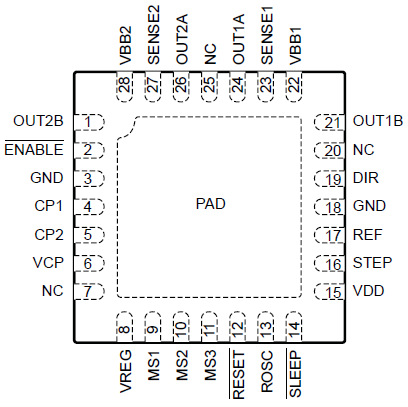
\includegraphics[scale = 0.75]{figuras/driverportas}
\caption{Portas do driver A4988.}
\caption*{Fonte: www.alldatasheet.com}
\label{fig:driverportas}
\end{figure}
    
% Tabela 1
\begin{table}[H]
    \footnotesize
    \centering
    \caption{Lista de terminais do driver A4988.}
    \begin{tabular}{lcl}
        \hline
        \textbf{Nome} & \textbf{Número} & \textbf{Descrição}\\
        \hline
         CP1 & 4 & Terminal do capacitor do pulso de carga\\
         CP2 & 5 & Terminal do capacitor do pulso de carga\\
         VCP & 6 & Terminal do capacitor do reservatório\\
         VREG & 8 & Terminal de desacoplamento regulador\\
         MS1 & 9 & Entrada lógica\\
         MS2 & 10 & Entrada lógica\\
         MS3 & 11 & Entrada lógica\\
         RESET & 12 & Entrada lógica\\
         ROSC & 13 & Ajuste de tempo\\
         SLEEP & 14 & Entrada lógica\\
         VDD & 15 & Fonte lógica\\
         STEP & 16 & Entrada lógica\\
         REF & 17 & Entrada de tensão de referência Gm\\
         GND & 3, 18 & Terra\\
         DIR & 19 & Entrada lógica\\
         OUT1B & 21 & DMOS ponte completa 1 saída B\\
         VBB1 & 22 & Abastecimento de carga\\
         SENSE1 & 23 & Ponte terminal do resistor do sensor 1\\
         OUT1A & 24 & DMOS ponte completa 1 saída A\\
         OUT2A & 26 & DMOS ponte completa 2 saída A\\
         SENSE2 & 27 & Ponte terminal do resistor do sensor 2\\
         VBB2 & 28 & Abastecimento de carga\\
         OUT2B & 1 & DMOS ponte completa 2 saída B\\
         ENABLE & 2 & Entrada lógica\\
         NC & 7, 20, 25 & Sem conexão\\
         PAD & - & Pasta térmica para dissipação aprimorada\\
        \hline       
    \end{tabular}
    \caption*{Fonte: www.alldatasheet.com.}
    \label{tab:pdriverportas}
\end{table}


\subsection{Atuadores}\label{subsec:metatuadores}

Atuadores são equipamentos ou dispositivos elétricos que convertem energia hidráulica, pneumática 
ou elétrica em energia mecânica. A energia gerada nos atuadores é transformada em movimento em 
vários tipos de processos.

Os atuadores utilizados neste projeto foram os elétricos que se dividem em  motores elétricos de 
corrente alternada e contínua, servomotores e motores de passo. Esses atuadores convertem pulsos 
elétricos recebidos em seus terminais em energia mecânica transformando-a em movimento rotativo 
do motor, no caso do projeto os motores de passo que controlam o movimento dos fusos da mesa 
cartesiana. Os atuadores elétricos atendem a comandos manuais ou programáveis, localmente ou remotamente. 
Eles se destacam por uma transmissão de potência simplificada e eficiente do ponto de vista de energia.

Os motores de passo são atuadores eletromagnéticos com capacidade de converter pulsos elétricos digitais 
recebidos em movimento de rotação incremental do eixo do motor. Sua aplicação é necessária em movimentos 
rotativos com alta precisão que necessitam de controle de posição e velocidade. A sua escolha foi definida 
pela precisão, baixo custo de aquisição e manutenção.

A composição de um motor de passo contém um rotor e um estator que é a parte fixa do gerador elétrico,
nessa está situado um conjunto de bobinas responsáveis pelo giro do rotor. Para que haja o movimento, 
as bobinas estão ligadas aos terminais do motor, organizadas em pares, interligadas entre si e 
posicionadas em sentidos opostos para que quando forem energizadas, der o movimento de rotação 
do motor devido às interações magnéticas.

O atributo que distingue o motor de passo dos demais motores elétricos é a capacidade de realizar passos, 
que são rotações discretas incrementais e precisas. Os passos são definidos por um número fixo de 
pólos magnéticos de dente de engrenagens do motor determinando assim, a precisão de ângulo de rotação 
do motor de passo. Para que haja um controle de quantos passos serão dados, o motor necessita de 
largura de pulso a fim de enviar a corrente adequada para cada passo. A Figura \ref{fig:didaticopasso} 
é um exemplo para melhor entendimento do conceito de passo.

\begin{figure}[H]
\centering
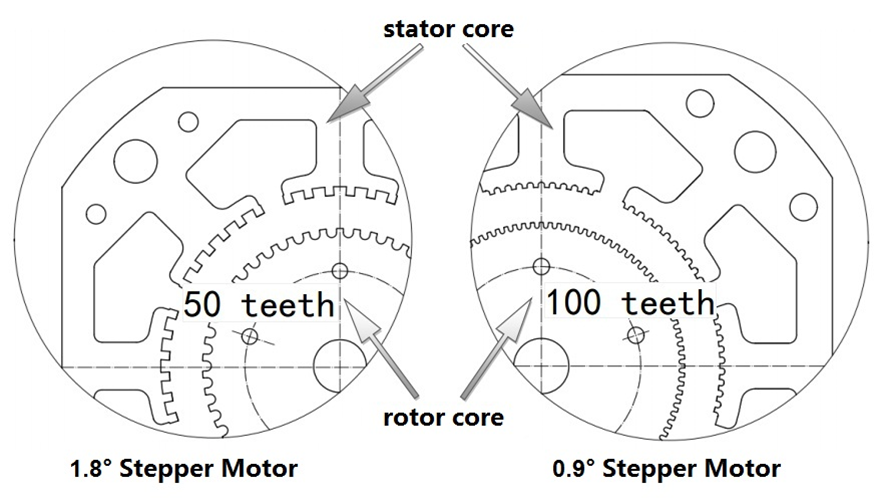
\includegraphics[scale = 0.4]{figuras/didaticopasso}
\caption{Conceito didático do motor de passo.}
\caption*{Fonte: https://www.fernandok.com.}
\label{fig:didaticopasso}
\end{figure}
    
A Figura \ref{fig:didaticopasso} mostra um motor de passo com 50 dentes de precisão, portanto combinando 
o número de dentes com as 4 fases de um motor bipolar temos 200 passos. 

A equação \ref{eq:Npassos} calcula o número de passos de uma volta executada pelo motor onde,
o número de passos ($n_{p}$) é igual ao número de dentes ($n_{d}$) multiplicado pelo número de fases ($n_{f}$)
\begin{equation}\label{eq:Npassos}
    n_{p} = n_{d} \cdot n_{f}
\end{equation}

A precisão do motor é definida por 360° divididos pelo número de passos. Portanto, 
360 divididos por 200 é igual a 1,8° de precisão. Já o segundo motor 
de passo possui 100 dentes de precisão, portanto a precisão é de 0,9°, o que indica que 
é um motor com maior precisão que o de 50 dentes.

Para aumentar a precisão dos motores é possível subdividir o passo de um motor em menores passos fornecendo 
ao mesmo tempo corrente elétrica em duas fases. Essa forma de trabalho é chamada de micropassos.

Logo, quando é fornecido a mesma magnitude de corrente a duas fases, um campo magnético de mesma magnitude 
é gerado, resultando em um movimento angular com a metade do passo original, essa configuração é chamada de 
meio passo. Assim, ao aplicar magnitudes de corrente diferentes a duas fases, o rotor se desloca 
proporcionalmente ao campo eletromagnético mais forte.

Os motores de passo utilizados no projeto da mesa cartesiana possuem 5 kgf.cm de torque, passo de 1,8° e 
corrente máxima de 2 Ampères por fase. O incremento de rotação e o torque são definidos conforme o modo 
de excitação que pode ser por passo completo, meio passo e micropasso explicadas anteriormente. O passo 
é dividido em quatro, oito ou dezesseis na maioria das vezes, mas também, atualmente se encontra 
sistemas capazes de dividir um passo em milhares de vezes.

\begin{figure}[H]
\centering
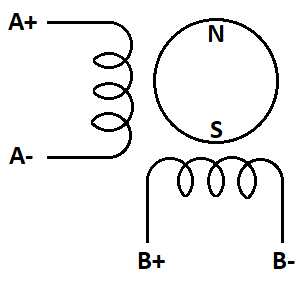
\includegraphics[scale = 0.6]{figuras/meumotorbipolar}
\caption{Esquema elétrico do motor de passo.}
\caption*{Fonte: Próprio autor.}
\label{fig:meumotorbipolar}
\end{figure}
    
As Tabelas \ref{tab:wavestephorario}, \ref{tab:fullstephorario} e \ref{tab:halfstephorario} 
mostram a sequência de polaridades aplicadas no motor no movimento de sentido horário.

% Tabela 2
\begin{table}[H]
    \footnotesize
    \centering
    \caption{Sequência de passos com uma fase (wavestep) para movimentação no sentido horário.}
    \begin{tabular}{cccccc}
        \hline
        \textbf{Passo} & \textbf{A+} & \textbf{B+} & \textbf{A-} & \textbf{B-} & \textbf{Decimal}\\
        \hline
        1 & 0 & 0 & 0 & 1 & 1\\
        2 & 0 & 0 & 1 & 0 & 2\\
        3 & 0 & 1 & 0 & 0 & 4\\
        4 & 1 & 0 & 0 & 0 & 8\\        
        \hline       
    \end{tabular}
    \caption*{Fonte: Próprio Autor, 2021.}
    \label{tab:wavestephorario}
\end{table}

% Tabela 3
\begin{table}[H]
    \footnotesize
    \centering
    \caption{Sequência de passos com duas fases (fullstep) para movimentação no sentido horário.}
    \begin{tabular}{cccccc}
        \hline
        \textbf{Passo} & \textbf{A+} & \textbf{B+} & \textbf{A-} & \textbf{B-} & \textbf{Decimal}\\
        \hline
        1 & 1 & 0 & 0 & 1 & 9\\
        2 & 0 & 0 & 1 & 1 & 3\\
        3 & 0 & 1 & 1 & 0 & 6\\
        4 & 1 & 1 & 0 & 0 & 12\\
        \hline       
    \end{tabular}
    \caption*{Fonte: Próprio Autor, 2021.}
    \label{tab:fullstephorario}
\end{table}

% Tabela 4
\begin{table}[H]
    \footnotesize
    \centering
    \caption{Sequência de passos com meio passo (halfstep) para movimentação no sentido horário.}
    \begin{tabular}{cccccc}
        \hline
        \textbf{Passo} & \textbf{A+} & \textbf{B+} & \textbf{A-} & \textbf{B-} & \textbf{Decimal}\\
        \hline
        1 & 1 & 0 & 0 & 1 & 9\\
        2 & 0 & 0 & 0 & 1 & 1\\
        3 & 0 & 0 & 1 & 1 & 3\\
        4 & 0 & 0 & 1 & 0 & 2\\
        5 & 0 & 1 & 1 & 0 & 6\\
        6 & 0 & 1 & 0 & 0 & 4\\
        7 & 1 & 1 & 0 & 0 & 12\\
        8 & 1 & 0 & 0 & 0 & 8\\
        \hline       
    \end{tabular}
    \caption*{Fonte: Próprio Autor, 2021.}
    \label{tab:halfstephorario}
\end{table}

As Tabelas \ref{tab:wavestepantihorario}, \ref{tab:fullstepantihorario} e \ref{tab:halfstepantihorario} 
mostram a sequência de polaridades aplicadas no motor no movimento de sentido anti-horário.

% Tabela 5
\begin{table}[H]
    \footnotesize
    \centering
    \caption{Sequência de passos com uma fase (wavestep) para movimentação no sentido anti-horário.}
    \begin{tabular}{cccccc}
        \hline
        \textbf{Passo} & \textbf{A+} & \textbf{B+} & \textbf{A-} & \textbf{B-} & \textbf{Decimal}\\
        \hline
        1 & 1 & 0 & 0 & 0 & 8\\
        2 & 0 & 1 & 0 & 0 & 4\\
        3 & 0 & 0 & 1 & 0 & 2\\
        4 & 0 & 0 & 0 & 1 & 1\\
        \hline       
    \end{tabular}
    \caption*{Fonte: Próprio Autor, 2021.}
    \label{tab:wavestepantihorario}
\end{table}

% Tabela 6
\begin{table}[H]
    \footnotesize
    \centering
    \caption{Sequência de passos com duas fases (fullstep) para movimentação no sentido anti-horário.}
    \begin{tabular}{cccccc}
        \hline
        \textbf{Passo} & \textbf{A+} & \textbf{B+} & \textbf{A-} & \textbf{B-} & \textbf{Decimal}\\
        \hline
        1 & 1 & 1 & 0 & 0 & 12\\
        2 & 0 & 1 & 1 & 0 & 6\\
        3 & 0 & 0 & 1 & 1 & 3\\
        4 & 1 & 0 & 0 & 1 & 9\\
        \hline       
    \end{tabular}
    \caption*{Fonte: Próprio Autor, 2021.}
    \label{tab:fullstepantihorario}
\end{table}

% Tabela 7
\begin{table}[H]
    \footnotesize
    \centering
    \caption{Sequência de passos com meio passo (halfstep) para movimentação no sentido anti-horário.}
    \begin{tabular}{cccccc}
        \hline
        \textbf{Passo} & \textbf{A+} & \textbf{B+} & \textbf{A-} & \textbf{B-} & \textbf{Decimal}\\
        \hline
        1 & 1 & 0 & 0 & 0 & 8\\
        2 & 1 & 1 & 0 & 0 & 12\\
        3 & 0 & 1 & 0 & 0 & 4\\
        4 & 0 & 1 & 1 & 0 & 6\\
        5 & 0 & 0 & 1 & 0 & 2\\
        6 & 0 & 0 & 1 & 1 & 3\\
        7 & 0 & 0 & 0 & 1 & 1\\
        8 & 1 & 0 & 0 & 1 & 9\\
        \hline       
    \end{tabular}
    \caption*{Fonte: Próprio Autor, 2021.}
    \label{tab:halfstepantihorario}
\end{table}

A Tabela \ref{tab:pmotordepasso} apresenta alguns parâmetros dos motores de passo.

% Tabela 8
\begin{table}[H]
    \footnotesize
    \centering
    \caption{Parâmetros dos motores de passo.}
    \begin{tabular}{ll}
        \hline
        \textbf{Parâmetros} & \textbf{Magnitude}\\
        \hline
        Número de passos por revolução & 200 (1,8 graus por passo)\\
        Corrente de operação & 800~mA\\
        Tensão de alimentação & 12~V\\
        Configuração das bobinas & Bipolar (4 fios)\\
        \hline       
    \end{tabular}
    \caption*{Fonte: Próprio Autor, 2021.}
    \label{tab:pmotordepasso}
\end{table}

\subsection{Fonte de alimentação}\label{subsec:metfonte}

A fonte de alimentação projetada para transformar a tensão elétrica alternada em corrente contínua.

Para a escolha correta da fonte de alimentação é necessário definir a demanda de energia elétrica 
que os dispositivos que são alimentados pela fonte necessitam.

A Tabela \ref{tab:demandafonte} apresenta a demanda de energia elétrica de cada dispositivo.

% Tabela 9
\begin{table}[H]
    \footnotesize
    \centering
    \caption{Demanda de energia elétrica de cada componente do sistema.}
    \begin{tabular}{lclll}
        \hline
        \textbf{Componente} & \textbf{Quantidade} & \textbf{Tensão} & \textbf{Consumo} & \textbf{Consumo Total}\\
        \hline
        Arduino & 1 & 7 a 12~V & 800~mA & 800~mA\\
        Driver & 2 & 8 a 35~V & 2~A & 4~A\\
        Motor de passo & 2 & 5 a 36~V & 2~A & 4~A\\
        Optoacoplador & 2 & 5 a 35~V & 5~mA & 10~mA\\
        Resultado & - & 12~V & - & 8,18~A\\
        \hline       
    \end{tabular}
    \caption*{Fonte: Próprio Autor, 2021.}
    \label{tab:demandafonte}
\end{table}

A Tabela \ref{tab:demandafonte} indica que a placa controladora Arduino opera no intervalo de tensão de 7~V 
a 12~V, os drivers de potência no intervalo de 8~V a 35~V, os motores de passo no intervalo de 5~V a 36~V 
e o optoacoplador no intervalo de 5~V a 35~V. A tensão de saída de 12~V foi determinada como melhor 
opção para o projeto.

Outro parâmetro que a Tabela \ref{tab:demandafonte} apresenta é a corrente elétrica mínima para a operação 
do circuito. A placa controladora necessita de 800~mA, os drivers de potência necessitam de 2~A cada, 
como são 2 drivers, 4~A são necessários, os motores de passo consomem 2 amperes cada, como o projeto 
contém 2 motores, 4 Amperes são necessários e os optoacopladores necessitam de 10~mA cada, como o 
projeto contém 2 optoacopladores, 20~mA são necessários. Decidiu-se acrescentar uma margem de 
segurança adicional de 30\% na corrente, então, considerou-se uma corrente mínima necessária de 10,64~A.

A equação \ref{eq:CorrenteNecessaria} calcula a demanda total de 
corrente elétrica mínima para a operação do circuito onde:
demanda total ($d_{total}$), demanda do arduino ($d_{arduino}$), demanda do driver de potência ($d_{driver}$),
demanda do motor de passo ($d_{motor}$) e demanda do optoacoplador ($d_{opto}$).

\begin{equation}\label{eq:CorrenteNecessaria}
    d_{total} = 1,3 \cdot (d_{arduino} + 2 \cdot d_{driver} + 2 \cdot d_{motor} + 2 \cdot d_{opto})    
\end{equation}

Conforme a determinação da tensão de saída e o cálculo de corrente necessária, 
é possível determinar que a fonte deve ter 12~V e 10,64~A.

\begin{figure}[H]
\centering
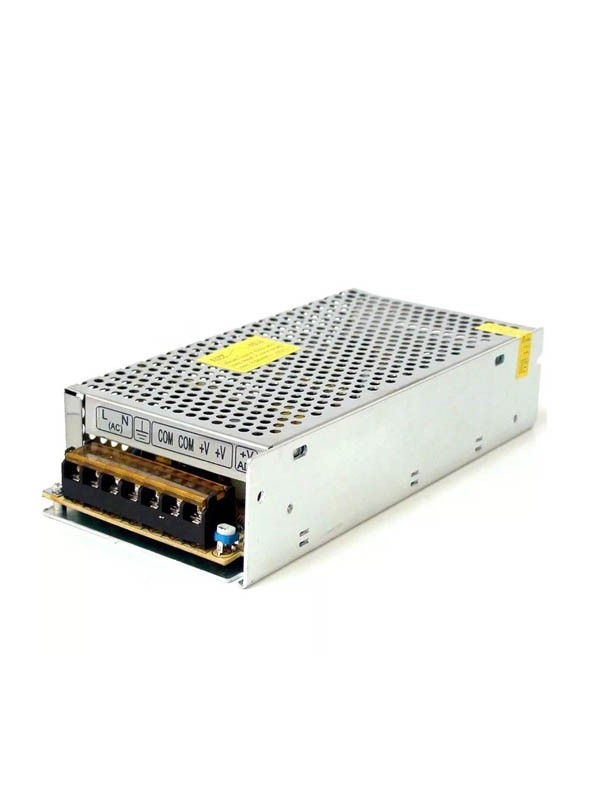
\includegraphics[scale = 0.6]{figuras/fonte}
\caption{Fonte do sistema.}
\caption*{Fonte: Próprio autor.}
\label{fig:fonte}
\end{figure}
    
\subsection{Acopladores ópticos}\label{subsec:metacoplador}

Os acopladores ópticos ou optoacopladores são dispositivos que realizam a transferência de 
sinais de um circuito para outro por meio de um feixe de luz sem a ligação elétrica.

A aplicação dentro do projeto é o isolamento elétrico que pode ser estabelecido entre 
os circuitos de controle de potência, protegendo os circuitos sensíveis a uma alta tensão 
como a placa controladora Arduino.

\begin{figure}[H]
\centering
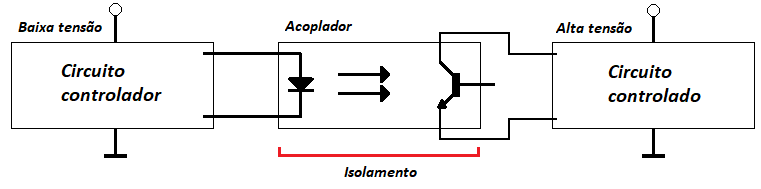
\includegraphics[width = 1\linewidth]{figuras/acoplador}
\caption{Funcionamento do acoplador no sistema.}
\caption*{Fonte: Próprio autor.}
\label{fig:acoplador}
\end{figure}
    
A sua composição contém uma fonte emissora de luz (LED) e um sensor fototransistor sensível às variações 
espectrais da fonte emissora. Seu funcionamento é baseado no efeito fotoelétrico, onde o diodo LED produz 
um feixe de luz infravermelha polarizando a base do fototransistor impondo uma condução entre base e emissor.

O optoacoplador escolhido para o projeto foi o PC 817 por já estar disponível no Laboratório de Sistemas 
Térmicos.

\subsection{Encoders}\label{subsec:metencoder}

Geradores de pulsos ou encoders são sensores/transdutores eletromecânicos responsáveis pelo sistema de 
controle de posição transformando a medida de posição de algum objeto, seja linear ou angular, em sinal 
elétrico digital que é transmitida à placa controladora, também conseguem converter movimentos circulares 
ou lineares em pulso elétricos.

Um encoder tem a capacidade de quantização de distâncias, controle de velocidades, medição de ângulos, 
medição de posição, medição de deslocamento relativo e etc. Sua composição contém um disco com marcações, 
um emissor e um receptor. Conforme o disco gira, vão sendo contadas às marcações e o emissor envia um sinal 
à placa controladora que por sua vez executa cálculos de distâncias, velocidades, ângulos, número de rotações 
e etc.

O princípio de funcionamento é dividido em três tipos, sendo eles: tacômetro, incremental e absoluto.

O encoder do tipo tacômetro possui um sinal de saída digital responsável em emitir um pulso para cada 
incremento captado no deslocamento. Este é utilizado na medição de velocidade e também no deslocamento 
angular unidirecional. O encoder incremental conta com sistema eletrônico externo responsável pela 
interpretação de posição, este dispositivo utiliza dois ou mais elementos geradores de sinal possuindo 
a capacidade de rotacionar por quantas revoluções forem necessárias.

E o encoder absoluto utiliza várias faixas de saídas com leitura em paralelo e são limitados a uma revolução. 
Os dados podem ser recuperados, se uma falha no sistema ocorrer, devido a representação binária da posição 
angular do eixo.

\subsection{Chaves fim de curso}\label{subsec:metchaves}

%PRECISA COLOCAR REFERENCIA \cite{alciatore2014introduccao}
As chaves fim de curso são dispositivos eletromecânicos usados para limitação de campo de movimento de eixos, 
como os presentes na mesa cartesiana. Esses componentes têm a capacidade de mudança de estado de conexão 
em circuitos, alternando o estado de aberto para fechado e vice-versa \cite{alciatore2014introduccao}. 
Seu estado inicialmente pode ser tanto normalmente aberto como normalmente fechado alterando seu estado 
por pino, gatilho, roldana, haste alavanca, etc. 

Uma chave fim de curso é composta basicamente por três elementos, sendo eles:

\begin{alineas}
    \item \textbf{Caixa:} Pode ser metálica ou plástica, dependendo do tipo e abriga os contatos e o atuador.
    \item \textbf{Contato:} É usado dentro do circuito a fim de fazer com que a atuação da chave fim de curso interrompa ou 
    acione algum outro dispositivo.
    \item \textbf{Atuador:} Recebe a força externa exercida para o acionamento da troca de estado.
\end{alineas}

\section{Sistema de software}\label{sec:metsissof}

A seguir será descrito o desenvolvimento do sistema de software.

%ABREVIATURA DE IDE
\subsection{Plataforma de prototipação Arduino IDE}\label{subsec:metide}

A plataforma de prototipação Arduino \ac{IDE} é um software que permite o desenvolvimento e envio 
de códigos compilados direto para o microcontrolador. Essa plataforma tem a flexibilidade de 
ser utilizada em vários sistemas operacionais e foi desenvolvida na linguagem Java oferecendo 
suporte de desenvolvimento na linguagem C e C++. O download da plataforma foi realizado 
através do link: https://www.arduino.cc/en/software

% Figura 3.19
\begin{figure}[H]
\centering
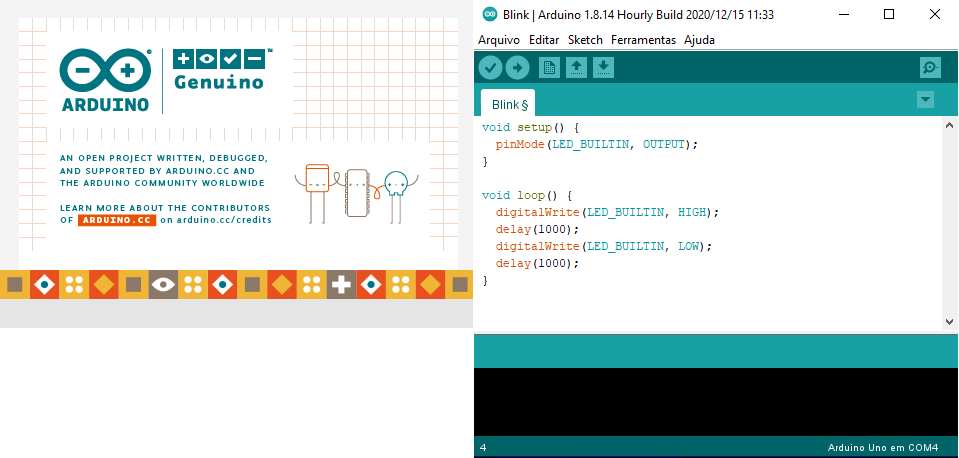
\includegraphics[width = 1\linewidth]{figuras/idearduino}
\caption{Ambiente de desenvolvimento integrado Arduino.}
\caption*{Fonte: Próprio autor.}
\label{fig:idearduino}
\end{figure}
    
\subsection{Logica de programação}\label{subsec:metlogica}

O desenvolvimento da lógica de programação da placa controladora foi organizado de maneira modular 
usando orientação a objetos para uma manutenção facilitada e um entendimento mais claro do código.

As operações que o software deve executar foram apresentadas no fluxograma abaixo.

\begin{figure}[H]
\centering
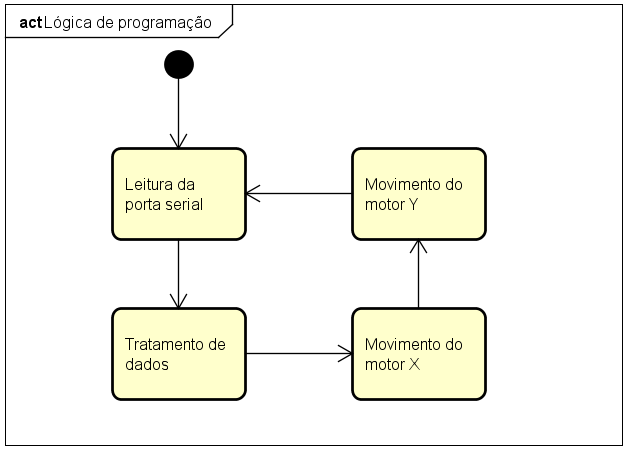
\includegraphics[width = 1\linewidth]{figuras/fluxoexecucao}
\caption{Fluxo de execução do software.}
\caption*{Fonte: Próprio autor.}
\label{fig:fluxoexecucao}
\end{figure}
    
A Figura \ref{fig:fluxoexecucao} apresenta um fluxograma simplificado da lógica de programação presente 
na placa controladora Arduino que inicialmente tem como primeiro comando ficar esperando o envio de 
dados pela porta Serial, se caso há esse envio, então o programa faz a leitura da porta serial, 
armazenando os dados em variáveis para em seguida realizar o tratamento de dados. Após o tratamento 
de dados o software dará o comando de movimentação do motor que controla o fuso do eixo horizontal 
(eixo X), em seguida, assim que o motor do eixo X parar sua rotação, o comando de movimentação 
do motor do eixo vertical (eixo Y) será acionado. Finalmente, após o fim da execução do motor 
que controla o eixo Y, o software volta a analisar se é enviado dados pela porta serial.

\subsection{Diagrama de classes}\label{subsec:metdiagrama}

Diagrama de classe é uma representação da estrutura e relações entre classes que um software possui 
facilitando e servindo de modelo para criação de objetos. Esse diagrama permite modelar classes com seus 
atributos e métodos além da relação entre objetos.

Para o desenvolvimento do software da placa controladora cuja linguagem é C++ que é fundamentada em 
orientação a objetos, foi definido que seria a melhor opção realizar um diagrama de classes antes do 
desenvolvimento do código. Sendo assim a Figura \ref{fig:diagramaclasses} apresentada abaixo é 
o resultado do que foi modelado.

\begin{landscape}
\begin{figure}[H]
\centering
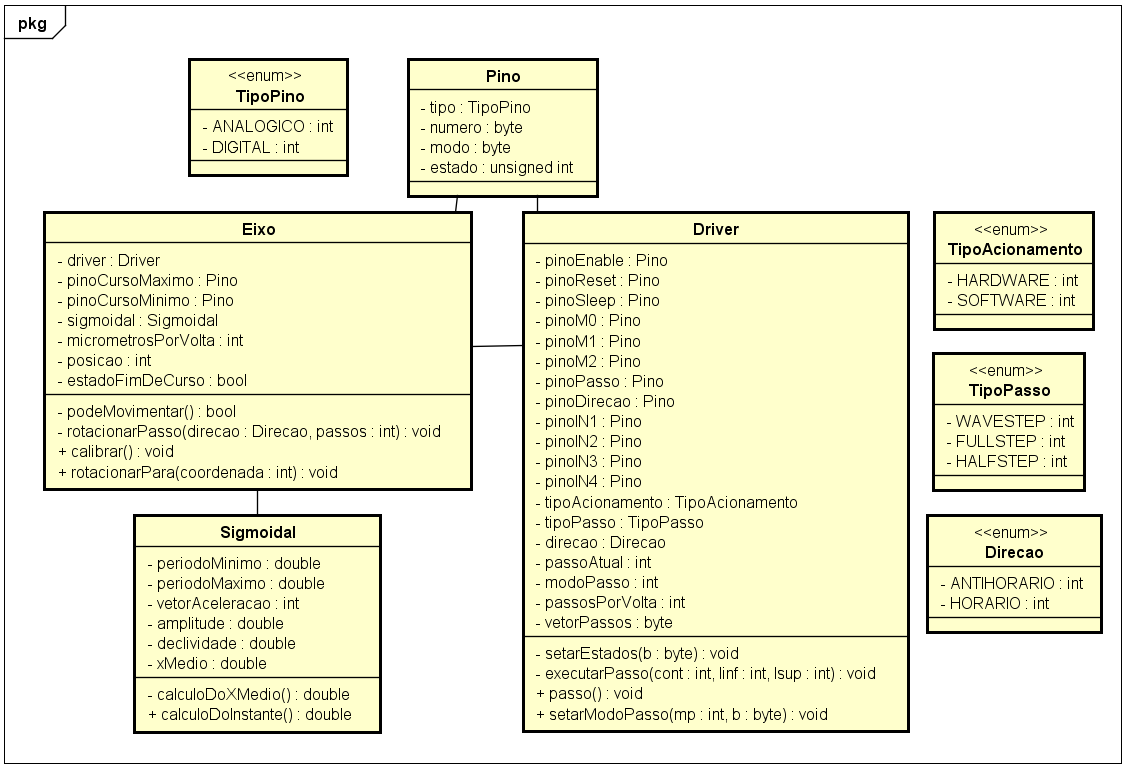
\includegraphics[scale = 0.65]{figuras/diagramaclasses}
\caption{Diagrama de classes do sistema de software presente no Arduino.}
\caption*{Fonte: Próprio autor.}
\label{fig:diagramaclasses}
\end{figure}
\end{landscape}

A seguir será explicado este diagrama classe a classe.

“Sigmoidal” é a classe responsável pela aceleração sigmóide nos motores de passo, essa classe utiliza 
a função sigmóide que é uma função matemática com o gráfico parecido com a letra S. Para o desenvolvimento 
da mesa cartesiana houve a preocupação dos projetistas em configurar os motores de passo com uma aceleração 
variável para maior vida útil dos equipamentos, já que com aceleração constante pode causar forças 
desnecessárias durante o processo de rotação.

A Tabela \ref{tab:classesigmoidal} apresenta a declaração e funcionalidade dos atributos e métodos 
da classe “Sigmoidal”.

% Tabela 10
\begin{table}[H]
    \footnotesize
    \centering
    \caption{Declaração e funcionalidade dos atributos e métodos da classe Sigmoidal.}
    \begin{tabular}{lp{9cm}}
        \hline
        \textbf{Declaração} & \textbf{Funcionalidade}\\
        \hline
        - periodoMinimo: double & Período máximo do passo do motor.\\
        - periodoMaximo: double & Período mínimo do passo do motor.\\
        - vetorAceleracao: int & Determina se a curva será de aceleração (1) ou desaceleração (-1)\\
        - amplitude: double & Amplitude da aceleração, diferença do período máximo menos o período mínimo\\
        - declividade: double & Inclinação da curva de aceleração, o quão rápido o motor irá acelerar\\
        - xMedio: double & É a metade do número de iterações necessários para percorrer a curva sigmoidal\\
        - calculoDoXMedio(): double & Calcula o número de Iterações necessários para percorrer metade da curva sigmoidal.\\
        + calculoDoInstante(): double & Calcula um instante na curva tendo como entrada uma iteração\\
        \hline       
    \end{tabular}
    \caption*{Fonte: Próprio Autor, 2021.}
    \label{tab:classesigmoidal}
\end{table}

A classe “Sigmoidal” tem como atributos privados: “periodoMaximo” e o “periodoMinimo” que são os períodos 
que o motor sofrerá os pulsos nas bobinas, “vetorAceleracao” que determina se a curva sigmoidal terá 
um comportamento de aceleração ou desaceleração, “amplitude” que é a diferença entre o “periodoMaximo” 
e o “periodoMinimo” e é utilizada na equação do cálculo do X médio e do cálculo do instante, “declividade” 
que determina a inclinação da curva de aceleração (o quão rápido o motor irá acelerar), “xMedio” que é a 
metade do número de passos (iterações) que o motor precisará para acelerar e é utilizado no cálculo 
do instante. 

Como operações, a classe “Sigmoidal” tem os métodos de acesso getters e setters que acessam os atributos 
privados citados acima, esses métodos são necessários para cumprir o princípio de encapsulamento da orientação 
a objetos protegendo a lógica da classe. A classe “Sigmoidal” dispõe de duas operações, as quais são definidas 
por: “calculoDoXMedio”, que calcula o valor do atributo xMedio, “calculoDoInstante”, que calcula o período a 
ser aplicado em um determinado instante, esse cálculo é utilizado na lógica do método “rotacionarPasso” 
da classe “Eixo”.

“Pino” é a classe que representa os pinos da placa Arduino, pois devido ao número alto de vezes que foi 
necessário a utilização dos pinos, foi definido que seria melhor a criação de uma classe para facilitar 
as operações com pinos. 

A Tabela \ref{tab:classepino} apresenta a declaração e funcionalidade dos atributos e métodos da 
classe “Pino”.

% Tabela 11
\begin{table}[H]
    \footnotesize
    \centering
    \caption{Declaração e funcionalidade dos atributos e métodos da classe Pino.}
    \begin{tabular}{lp{9cm}}
        \hline
        \textbf{Declaração} & \textbf{Funcionalidade}\\
        \hline
        - tipo: TipoPino & Tipo do pino (ANALOGICO, DIGITAL).\\
        - numero: byte & Número do pino.\\
        - modo: byte & Modo do pino (OUTPUT, INPUT).\\
        - estado: unsigned int & Estado do pino (LOW, HIGH) | (0, 255) | (0, 1023).\\
        \hline       
    \end{tabular}
    \caption*{Fonte: Próprio Autor, 2021.}
    \label{tab:classepino}
\end{table}

A classe “Pino” possui como atributos privados: “tipo”, que é o tipo de entrada do pino que pode ser 
analogico ou digital, “numero”, que é o número de uma determinada porta na placa, “modo” que define se 
a porta é de entrada ou saída de dados, e “estado”, que pode estar ligado ou desligado nas portas digitais, 
ter valores de 0 a 255 nas portas \ac{PWM} e de 0 a 1023 nas portas analogicas. Como operações, a classe “Pino” 
tem os métodos de acesso getters e setters que acessam os atributos privados citados acima.

“Driver” é a classe responsável pelo controle digital do driver de potência, com ela é possível definir 
o modo do passo dos motores, executar o pulso que dará movimento ao motor de passo, ligar e desligar 
o driver, deixá-lo no modo “sleep” e também “reseta-lo”.

A Tabela \ref{tab:classedriver} apresenta a declaração e funcionalidade dos atributos e métodos da 
classe “Driver”

% Tabela 12
\begin{table}[H]
    \footnotesize
    \centering
    \caption{Declaração e funcionalidade dos atributos e métodos da classe Driver.}
    \begin{tabular}{p{8cm}p{6cm}}
        \hline
        \textbf{Declaração} & \textbf{Funcionalidade}\\
        \hline
        - pinoEnable: Pino & Ativar e desativar o driver.\\
        - pinoReset: Pino & Resetar o driver.\\
        - pinoSleep: Pino & Ativar e desativar o modo sleep do driver.\\
        - pinoM0: Pino & Pino M0 do modo de passo do driver.\\
        - pinoM1: Pino & Pino M1 do modo de passo do driver.\\
        - pinoM2: Pino & Pino M2 do modo de passo do driver.\\
        - pinoPasso: Pino & Pino de execução do passo do driver.\\
        - pinoDirecao: Pino & Pino de configuração da direção do driver.\\
        - pinoIN1: Pino & Pino IN1 do motor de passo.\\
        - pinoIN2: Pino & Pino IN2 do motor de passo.\\
        - pinoIN3: Pino & Pino IN3 do motor de passo.\\
        - pinoIN4: Pino & Pino IN4 do motor de passo.\\
        - tipoAcionamento: TipoAcionamento & Tipo de acionamento do~driver:~(SOFTWARE,~HARDWARE).\\
        - tipoPasso: TipoPasso & Tipo do passo do driver: (WAVESTEP, FULLSTEP, HALFSTEP).\\
        - direcao: Direcao & Configuração da direção do driver: (ANTIHORARIO, HORARIO).\\
        - passoAtual: int & PassoAtual é o indice de acesso as informações do vetor de passos.\\
        - modoPasso: int & Pino do modo de passo do driver.\\
        - passosPorVolta: int & Quantidade de passos a cada volta do motor de passo.\\
        - vetorPasso: byte & Vetor de bytes de sequência dos passos.\\
        - setarEstadoModo(pM0:bool, pM1:bool, pM2:bool):~void & Definir o modo de passo do driver passando como parâmetros o estado dos pinos M0, M1 e M2.\\
        - setarEstados(b: byte):void & Definir estados dos pinos IN1, IN2, IN3, IN4 do motor de passo.\\
        - passo():void & Executar um passo do motor.\\
        + executarPasso(cont:int, linf:int, lsup:int):void & Executar um passo do motor com a lógica de sequência dos passos.\\
        + setarModoPasso(mp:int, b:byte):void & Definir o modo de passo do driver.\\
        \hline       
    \end{tabular}
    \caption*{Fonte: Próprio Autor, 2021.}
    \label{tab:classedriver}
\end{table}

A classe “Driver” possui os atributos privados: “pinoEnable”, que permite ligar ou desligar o driver, 
“pinoReset”, que reinicia o driver, “pinoSleep”, que ativa o modo sleep do driver, “pinoM0”, “pinoM1” 
e “pinoM2”, que definem o modo do Passo, “pinoPasso” e “pinoDirecao” que são os pinos de execução de 
passo e configuração de direção para tipo de acionamento via hardware, “pinoIN1”, “pinoIN2”, “pinoIN3” 
e “pinoIN4” que são os pinos referentes ao controle das bobinas do motor de passo para tipo de acionamento 
via software, “tipoAcionamento” para configuração do tipo de acionamento do driver que pode ser via software 
ou hardware conforme a necessidade de cada tipo de driver utilizado, “tipoPasso” para configuração do tipo 
de passo do driver que pode ser (wavestep, fullstep, halfstep), “direcao”, que define o sentido do movimento, 
“passoAtual” que é o índice de acesso às informações do vetor de passos, “modoPasso”, que define o modo do 
passo do driver, “passosPorVolta”, que define a quantidade de passos a cada volta do motor como por exemplo, 
200 passos de 1,8° resultando em 360°. 

Como operações, a classe “Driver” tem os métodos: métodos de acesso getters e setters que acessam os 
atributos privados da classe, os métodos: “setarEstados”, que define os estados dos pinos IN1, IN2, IN3, 
IN4 do motor de passo, “passo” que executa um passo do motor, “setarModoPasso”, que define o modo de passo 
do driver e “executarPasso”, executa um passo do motor com a lógica de configurações de passos.

“Eixo” é a classe que foi desenvolvida a lógica de movimentação dos eixos da mesa cartesiana. Com ela é 
possível rotacionar definindo a coordenada cartesiana de preferência, verificar se a posição do eixo 
está ativando a chave de fim de curso.

A Tabela \ref{tab:classeeixo} apresenta a declaração e funcionalidade dos atributos e métodos da 
classe “Eixo”.

% Tabela 13
\begin{table}[H]
    \footnotesize
    \centering
    \caption{Declaração e funcionalidade dos atributos e métodos da classe Eixo.}
    \begin{tabular}{lp{6cm}}
        \hline
        \textbf{Declaração} & \textbf{Funcionalidade}\\
        \hline
        - driver: Driver & Define as configurações do driver que controla os motores de passo.\\
        - sigmoidal: Sigmoidal & Define a aceleração sigmoidal dos motores de passo.\\
        - pinoCursoMinimo: Pino & Pino do curso mínimo da chave fim de curso.\\
        - pinoCursoMaximo: Pino & Pino do curso máximo da chave fim de curso.\\
        - posicao: int & Pino da posição atual do eixo.\\
        - estadoFimDeCurso: bool & Pino do estado de fim de curso que pode inicializar LOW ou HIGH.\\
        - podeMovimentar(direcao:bool):bool & Verificar se o motor está no fim de curso.\\
        - rotacionarPassos(direcao:bool,passos:int):void & Rotacionar o motor, tendo como parâmetros de entrada a direção e a quantidade de passos.\\
        + rotacionarPara(coordenada:double):void & Rotacionar o motor tendo como parâmetro a coordenada cartesiana do eixo.\\
        \hline       
    \end{tabular}
    \caption*{Fonte: Próprio Autor, 2021.}
    \label{tab:classeeixo}
\end{table}

A classe “Eixo” possui os atributos privados: “driver”, que é responsável pelas configurações e operações 
do driver de potência que controla o motor de passo acoplado ao eixo, “sigmoidal” que define a aceleração 
variável do motor, “pinoCursoMinimo” e “pinoCursoMaximo”, que são os pinos referentes às chaves fim de 
curso de cada eixo, “estadoFimDeCurso”, que indica o estado que a chave fim de curso inicializará estando 
desativada. 

Como operações, a classe tem os métodos: métodos de acesso getters e setters que acessam os atributos 
privados da classe, os métodos: “podeMovimentar”, que indica se o motor de passo pode executar o próximo 
passo ou se já chegou ao fim do curso, “rotacionarPassos”, que rotaciona o eixo tendo como parâmetros de 
entrada uma direção e uma quantidade de passos a serem executadas e “rotacionarPara”, que rotaciona o 
eixo tendo como parâmetros de entrada uma coordenada cartesiana.

Além das classes utilizadas, o software possui a \textit{sketch} principal que é responsável pela configuração das 
informações iniciais, criação dos objetos na memória, configuração dos atributos de cada objeto, execução 
da leitura pela porta serial, tratamento de dados recebidos e a movimentação dos motores.
A Figura \ref{fig:orgsoftware} apresenta um diagrama geral da organização do software.

\begin{figure}[H]
\centering
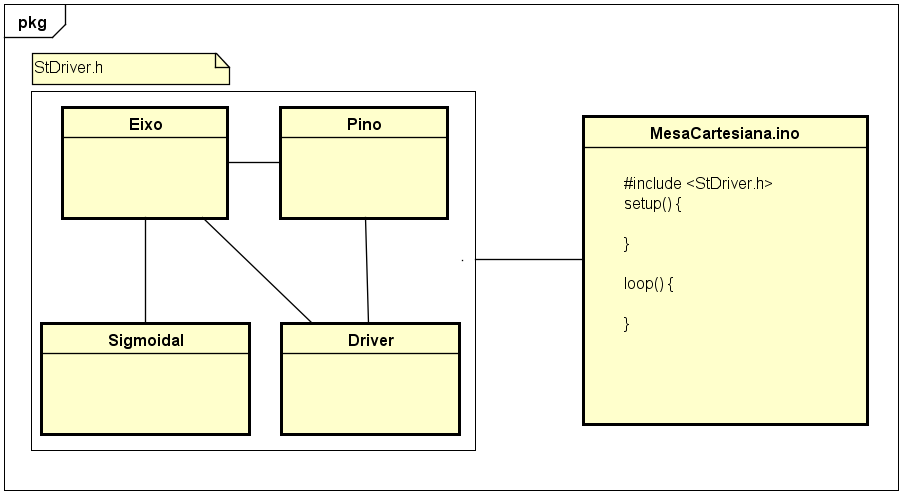
\includegraphics[width = 1\linewidth]{figuras/orgsoftware}
\caption{Diagrama da organização geral do software.}
\caption*{Fonte: Próprio autor.}
\label{fig:orgsoftware}
\end{figure}
    
O arquivo “MesaCartesiana.ino” é o principal, ele instancia os objetos das classes: “Pino”, “Sigmoidal”, 
“Driver” e “Eixo” e também tem a responsabilidade de receber às coordenadas através da comunicação serial 
e às enviar para o objeto da classe “Eixo” que fará a rotação dos motores.

\section{Integração dos sistemas}\label{subsec:metintegracao}

Nesta seção será descrito como os sistemas são integrados mostrando como os três sistemas se comunicam. 
A Figura \ref{fig:integracao} é um fluxograma que descreve de maneira gráfica a integração dos sistemas.

\begin{figure}[H]
\centering
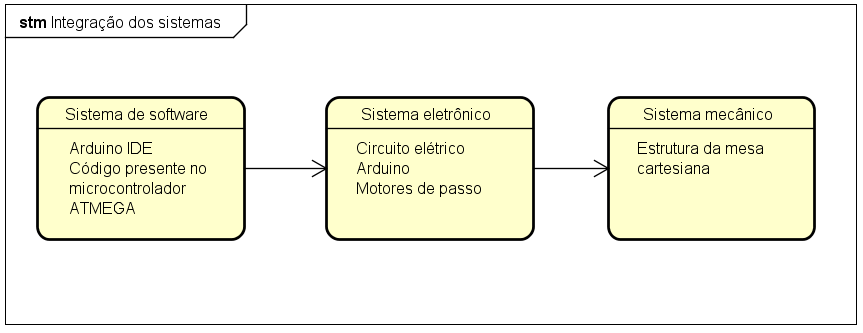
\includegraphics[width = 1\linewidth]{figuras/integracao}
\caption{Fluxograma para apresentar a integração dos sistemas.}
\caption*{Fonte: Próprio autor.}
\label{fig:integracao}
\end{figure}
    
O sistema de software se comunica com o sistema eletrônico através do envio de dados pela comunicação 
Serial presente no Arduino IDE para o software presente no microcontrolador ATMEGA da placa Arduino. 
Por sua vez, o microcontrolador envia um comando elétrico ao sistema eletrônico que acionará os motores 
de passo que convertem a energia elétrica em mecânica transmitindo o movimento dos fusos a estrutura do 
sistema mecânico.